\documentclass[tikz,border=2pt]{standalone}
\usepackage{amsmath}
\usepackage{pgfplots}
\pgfplotsset{compat=1.18}
\usetikzlibrary{arrows.meta}
\begin{document}
% A list holds elements of different type and size: l1 = list(A = "character", B = c(10L, 20L),
% C = 2 x 2 logical matrix); nothing is converted.
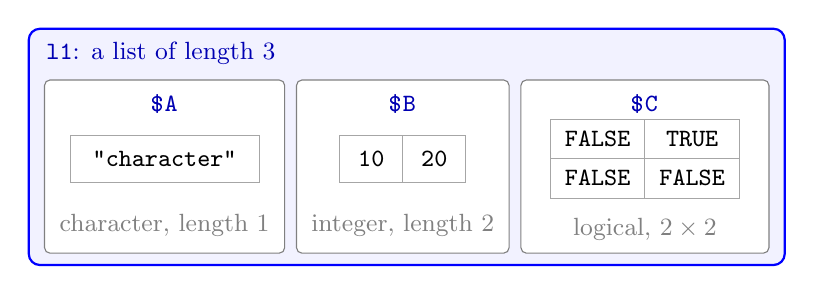
\begin{tikzpicture}[font=\small, >={Latex[length=2mm]},
  cell/.style={draw, gray!70, minimum height=6mm, inner sep=2pt, font=\small\ttfamily, text=black}]
  \draw[blue, thick, rounded corners=4pt, fill=blue!5] (0,0) rectangle (9.6,3.0);
  \node[anchor=north west, blue!70!black] at (0.1,2.95) {\texttt{l1}: a list of length 3};
  % compartment A
  \draw[gray, rounded corners=2pt, fill=white] (0.2,0.15) rectangle (3.25,2.35);
  \node[font=\small\ttfamily, blue!70!black] at (1.725,2.05) {\$A};
  \node[cell, minimum width=24mm] at (1.725,1.35) {"character"};
  \node[gray] at (1.725,0.5) {character, length 1};
  % compartment B
  \draw[gray, rounded corners=2pt, fill=white] (3.4,0.15) rectangle (6.1,2.35);
  \node[font=\small\ttfamily, blue!70!black] at (4.75,2.05) {\$B};
  \node[cell, minimum width=8mm] at (4.35,1.35) {10};
  \node[cell, minimum width=8mm] at (5.15,1.35) {20};
  \node[gray] at (4.75,0.5) {integer, length 2};
  % compartment C
  \draw[gray, rounded corners=2pt, fill=white] (6.25,0.15) rectangle (9.4,2.35);
  \node[font=\small\ttfamily, blue!70!black] at (7.825,2.05) {\$C};
  \node[cell, minimum width=12mm, minimum height=5mm] at (7.225,1.6) {FALSE};
  \node[cell, minimum width=12mm, minimum height=5mm] at (8.425,1.6) {TRUE};
  \node[cell, minimum width=12mm, minimum height=5mm] at (7.225,1.1) {FALSE};
  \node[cell, minimum width=12mm, minimum height=5mm] at (8.425,1.1) {FALSE};
  \node[gray] at (7.825,0.45) {logical, $2\times2$};
\end{tikzpicture}
\end{document}
